\subsubsection{Task Merging Algorithms}

\subsubsection{Power Interrupt Immune Scheduler}

% TNT :  Total Number of Tasks
% JT 	: Total Jump
% ID	: Task ID
% D	: relative Jump (Delta)
% VCT_PT : Current Task Pointer

% if(TJ < TNT)
% 	VCT_PT <- VCT_PT + D
% else
% 	while ((dis = TJ - TNT) > TNT)
% 		dis -= ID
% 	VCT_PT <- VCT_PT + dis


\begin{algorithm}[t]
	\caption{\sys's scheduler: relative jump algorithm}
	\label{algo:relativeJump}
	\scriptsize
	%\small
	\begin{algorithmic}[1]
			\State \textsf{TNT}: Total Number of Tasks
			\State \textsf{ID}: Task ID
			\State \textsf{$\delta$}: Relative Jump
			\State $\textsf{TJ} \leftarrow (\textsf{ID} + \delta )$ \Comment{Total Jump}
			\State \textsf{\textsf{$VCT_{pt}$}}: Virtual Current Task Pointer

			\If { \textsf{TJ} > \textsf{TNT} }
				\State $\textsf{dis} = \textsf{TJ} - \textsf{TNT}$
				\While{ $ \textsf{dis} > TNT $ }
					\State $\textsf{dis} -= \textsf{TNT}$
				\EndWhile
				\State $\textsf{dis} -= \textsf{ID}$
				\State \textsf{$VCT_{pt}$} $+= \textsf{dis}$
			\Else
				\State \textsf{$VCT_{pt}$} $+= \delta $

			\EndIf
	\end{algorithmic}
\end{algorithm}

It utilizes a persistent circular buffer (persistent linked-list) to keep the state of a program across power failures. \sys provides an API to enable a programmer to have a full control over the execution flow of the program, i.e. (un)blocking a task or re-execute the same task which is particularly important in the intermittent execution to emulate a persistent loop. 

\paragraph{Fixed Virtual Task Size}

	\begin{algorithm}[t]
		\caption{Fixed virtual Task size}
		\label{algo:fixVirtTask}
		\scriptsize
		%\small
		\begin{algorithmic}[1]
			\State $VT \subset \text{\{\sys Tasks\}} $  \Comment{$VT:$ Virtual Task}
			\State VTS : VT size
			\State MVTS: maximum VT size
			\vspace{0.1cm}

			\While {$True$}
				\State $VT \leftarrow VT_{next}$
				\vspace{0.1cm}
				\While {execute $VT$} 
					\If { $\text{power failed twice}$ }				
							\State $VTS--$  
							\State $ MVTS = VTS $
						\EndIf
				\EndWhile

				\vspace{0.1cm}
				\If {$ \text{All tasks executed}$}
					\If{$VTS < MVTS$}
					\State $VTS++$
					\EndIf
				\EndIf
			\EndWhile
		\end{algorithmic}
	\end{algorithm}


	\begin{algorithm}[t]
		\caption{Opportunistic virtual Task size}
		\label{algo:fixVirtTask}
		\scriptsize
		%\small
		\begin{algorithmic}[1]
			\State $VT \subset \text{\{\sys Tasks\}} $  \Comment{$VT:$ Virtual Task}
			\State VTS : VT size
			\vspace{0.1cm}

			\While {$True$}
				\State $VT \leftarrow VT_{next}$
				\vspace{0.1cm}
				\While {execute $VT$} 
					\If { $\text{power failed twice}$ }				
							\State $VTS--$  
						\EndIf
				\EndWhile

				\vspace{0.1cm}
				\If {$ \text{All tasks executed}$}
					\State $VTS++$
				\EndIf
			\EndWhile
		\end{algorithmic}
	\end{algorithm}

\begin{figure}[t]
	\centering
	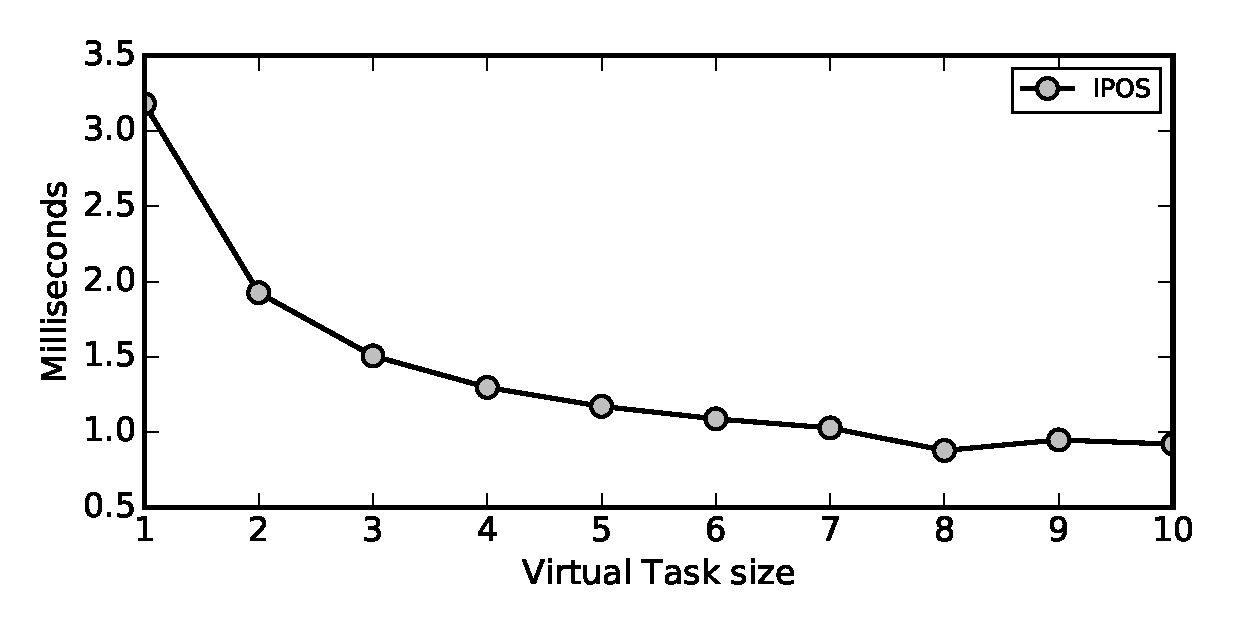
\includegraphics[width=0.8\columnwidth]{figures/virtualTaskSize.eps}
	\caption{Size of the virtual task versus the execution time of a dummy application that contains 12 empty tasks.}
	\label{fig:virtualTaskSize}
\end{figure}

\begin{figure}
	\centering
	%\includegraphics[width=0.25\columnwidth]{figures/task_coalescing}
	\caption{Task coalescing architecture.}
	\label{fig:}
\end{figure}

\sys is able to virtually merge tasks to construct a bigger virtual task and commit the state of the virtual task instead of the individual real tasks. 
Fig.~\ref{fig:virtualTaskSize} show the benefit of virtualizing the Modular Intermittent Execution Mode (MIEM) in the best case scenario (continuous power supply). 

Remark: A less obvious benefit of visualization is that it can enable a secure computation. By increasing the size of the virtual task, the energy in the super-capacitor will not be enough to finish the execution of the virtual task. Therefore, without the interrogator being close to the intermittently powered device and charging rate is not negligible as compared to the discharging rate this computation will not be finished. As such, virtualization can add a layer of security to the computation.